\chapter{OpenGL}
Ao longo do final do século XX, a computação gráfica ganhou grande importância na vida de pessoas comuns. Tal tecnologia se tornou presente não apenas em usos militares como SAGE (\textit{Semi-Automatic Ground Environment}), sistema que convertia dados de radares em imagens computadorizadas (MACHOVER, 1978) na década de 50, como também em filmes como Toy Story (1995) (figura \ref{fig:toy-story}), primeiro longa-metragem completamente computadorizado (GUHA, 2010).

\begin{figure}[h]
	\centering
	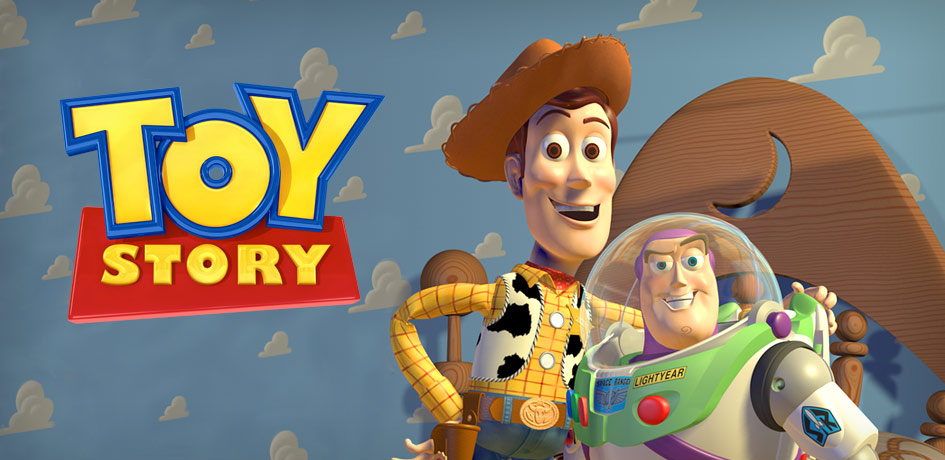
\includegraphics[scale=0.35]{imagens/toy-story.jpg}
	\caption{\small Filme Toy Story. (Fonte: Pixar, 2016)}
	\label{fig:toy-story}
\end{figure}

Na década de 80, boa parte do trabalho gráfico era produzido em \textit{workstations}, que utilizavam a APIs com diferentes implementações, dificultando a produção de programas multiplataforma. Em 1982, a SGI (Silicon Graphics, Inc) começou o desenvolvimento de sua API proprietária IRIS GL, atingindo alta popularidade (MARTZ, 2006). A pressão por uma API aberta e unificada aumentou por parte dos desenvolvedores de software, culminando em 1991 com a formulação do OpenGL ARB (\textit{Architecture Review Board}), consórcio de empresas para regulamentar o projeto, e o lançamento da versão 1.0 no ano seguinte.

Segundo Wright (2013), o OpenGL é uma camada de abstração entre o \textit{software} e o sistema gráfico, devendo permitir que a aplicação execute independente dos diferentes tipos de \textit{hardware}. Além disso, a API precisa operar em diferentes sistemas operacionais, arquiteturas e resoluções de tela, ao mesmo tempo que expõe as características de cada \textit{hardware} para que o programador faça o melhor uso.

Em 2004, com o lançamento da versão 2.0, foi lançada a OpenGL \textit{Shading Language},

Com o tempo, várias funções foram adicionadas a especificação, o que tornava difícil a compatibilidade entre todas elas. Por esse motivo, em 2008, o OpenGL ARB decidiu criar dois perfis: \textit{core} e \textit{compatibility}, separando padrões suportados por arquiteturas modernas e obsoletas, respectivamente.